\documentclass[final_report_innit.tex]{subfiles}

\begin{document}

\section{Results Analysis}

In this section, we will present our survey results, on the basis of which we hope to identify the applicability of process and design activities to the MC and MDSD paradigms. Our survey questions have provided us with data on five process and design activities: continuous integration (CI), cross-functional teams (CF), feature development (FD), unit testing (UT) and component testing (CT). We have measured the impact of these activities with regard to performance and productivity, quality of deliverables, personal fulfillment and ease of implementation.

The survey data came from twenty questionnaires which were sent to employees at Ericsson, specifically those working in the EPG department. Our contact at Ericsson distributed them between the MC and MDSD practitioners. We received fourteen replies, and out of those six were from the MDSD practitioners and eight from MC. Out of those responses we deemed that four responses from the MDSD practitioners were suitable and that seven from the MC practitioners were also suitable. Suitability was derived from how complete the answer sets were, for example, most of the responses which were stricken were missing well over 50\% of the answers and thus were unsuited for analysis.

When analysing the data we decided not to perform any complicated statistical analysis. The primary motivation for this was the small scale of the data set that we had collected; had we collected more, a proper statistical analysis might have been appropriate. To generate our averages, we simply calculated the mean responses from grouping of answers. We generated an average for each of MDSD and MC in relation to the design and process questions. We then generated an average of all the questions and finally generated averages from each question block for MDSD and MC ending with an average of both of these together.

The final part of the analysis involved an interview with our contact at Ericsson. The interview provided additional insight into some of the design and process elements which they utilise, especially those that we were particularly interested in.

With regard to cross-functional teams, the interviewee seemed to be in agreement with the positive responses of both MC and MDSD practitioners, since the interviewee indicated that their change is completed and part of the culture at EPG. However, considering the discrepancy of responses on continuous integration, the interviewee expressed that the discontent of MC practitioners was unexpected, since the interviewee believed that continuous integration should be as applicable to the MC paradigm as to the MDSD paradigm. Overall, the interview that we conducted with our contact at EPG helped us to formulate our assumptions about the survey results. 
%\usepackage{tkiz}

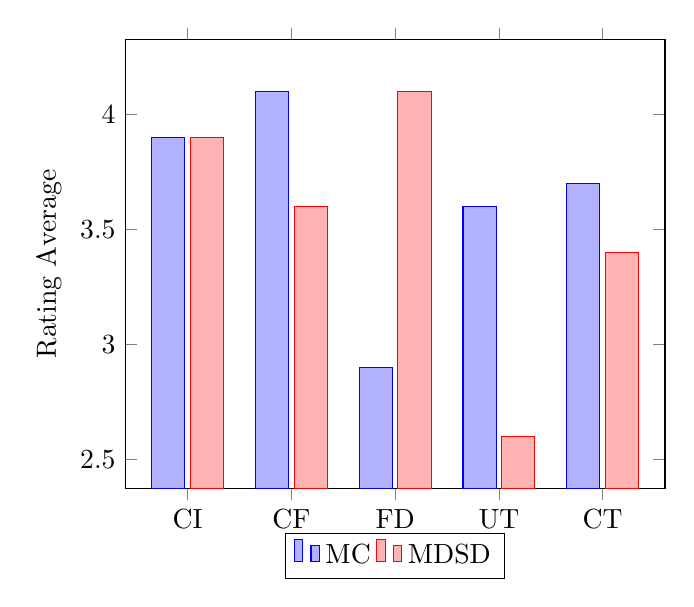
\begin{tikzpicture}
\begin{axis}[
	every axis plot post/.style={/pgf/number format/fixed},
	symbolic x coords={CI, CF, FD, UT, CT},
	ylabel=Rating Average,
	enlargelimits=0.15,
	legend style={at={(0.5,-0.1)},
	anchor=north,legend columns=-1},
	%ybar interval=0.7,
	ybar,
	bar width=12pt
]
\addplot 
	coordinates {(CI,3.9) (CF,4.1)
		 (FD,2.9) (UT,3.6) (CT,3.7)};
\addplot 
	coordinates {(CI,3.9) (CF,3.6) 
		(FD,4.1) (UT,2.6) (CT,3.4)};
\legend{MC,MDSD}
\end{axis}
\end{tikzpicture}

\textit{``Response Average of MC and MDSD respondents for Process and Design Activities''}


% Please add the following required packages to your document preamble:
% \usepackage{booktabs}
\begin{table}[h]
\caption{Process Activity Survey Results}
\centering
\begin{tabular}{@{}l|c|c|c|@{}}
\cmidrule(l){2-4}
                             & \multicolumn{1}{l|}{avg(MC)} & \multicolumn{1}{l|}{avg(MDD)} & \multicolumn{1}{l|}{avg(all)} \\ \midrule
\multicolumn{1}{|l|}{CI-P}   & 4.1                          & 4.0                           & 4.1                           \\ \midrule
\multicolumn{1}{|l|}{CI-Q}   & 3.6                          & 4.0                           & 3.7                           \\ \midrule
\multicolumn{1}{|l|}{CI-PF}  & 3.4                          & 3.0                           & 3.3                           \\ \midrule
\multicolumn{1}{|l|}{CI-EOI} & 4.3                          & 4.5                           & 4.4                           \\ \midrule
\multicolumn{1}{|l|}{CF-P}   & 4.3                          & 4.0                           & 4.3                           \\ \midrule
\multicolumn{1}{|l|}{CF-Q}   & 4.0                          & 1.0                           & 3.6                           \\ \midrule
\multicolumn{1}{|l|}{CF-PF}  & 3.7                          & 3.0                           & 3.5                           \\ \midrule
\multicolumn{1}{|l|}{CF-EOI} & 4.5                          & 5.0                           & 4.6                           \\ \midrule
\multicolumn{1}{|l|}{FD-P}   & 3.2                          & 4.0                           & 3.6                           \\ \midrule
\multicolumn{1}{|l|}{FD-Q}   & 3.2                          & 4.5                           & 3.8                           \\ \midrule
\multicolumn{1}{|l|}{FD-PF}  & 3.0                          & 3.0                           & 3.0                           \\ \midrule
\multicolumn{1}{|l|}{FD-EOI} & 2.2                          & 4.5                           & 3.2                           \\ \bottomrule
\end{tabular}
\end{table}


% Please add the following required packages to your document preamble:
% \usepackage{booktabs}
\begin{table}[h]
\caption{Design Activity Survey Results}
\centering
\begin{tabular}{@{}l|c|c|c|@{}}
\cmidrule(l){2-4}
                             & \multicolumn{1}{l|}{avg(MC)} & \multicolumn{1}{l|}{avg(MDD)} & \multicolumn{1}{l|}{avg(all)} \\ \midrule
\multicolumn{1}{|l|}{UT-P}   & 3.5                          & 3.0                           & 3.4                           \\ \midrule
\multicolumn{1}{|l|}{UT-Q}   & 4.0                          & 3.0                           & 3.8                           \\ \midrule
\multicolumn{1}{|l|}{UT-PF}  & 3.3                          & 3.0                           & 3.3                           \\ \midrule
\multicolumn{1}{|l|}{UT-EOI} & 3.5                          & 1.7                           & 2.9                           \\ \midrule
\multicolumn{1}{|l|}{CT-P}   & 3.7                          & 4.0                           & 3.8                           \\ \midrule
\multicolumn{1}{|l|}{CT-Q}   & 4.7                          & 5.0                           & 4.8                           \\ \midrule
\multicolumn{1}{|l|}{CT-PF}  & 3.0                          & 3.0                           & 3.0                           \\ \midrule
\multicolumn{1}{|l|}{CT-EOI} & 3.3                          & 2.5                           & 2.9                           \\ \bottomrule
\end{tabular}
\end{table}

% Please add the following required packages to your document preamble:
% \usepackage{booktabs}
\begin{table}[h]
\caption{Design and Process Group Averages}
\centering
\begin{tabular}{@{}c|c|c|c|@{}}
\cmidrule(l){2-4}
\multicolumn{1}{l|}{}    & \multicolumn{1}{l|}{avg/group(MC)} & \multicolumn{1}{l|}{avg/group(MDD)} & \multicolumn{1}{l|}{avg/group(all)} \\ \midrule
\multicolumn{1}{|c|}{CI} & 3.9                                & 3.9                                 & 3.9                                 \\ \midrule
\multicolumn{1}{|c|}{CF} & 4.1                                & 3.6                                 & 4.0                                 \\ \midrule
\multicolumn{1}{|c|}{FD} & 2.9                                & 4.1                                 & 3.4                                 \\ \midrule
\multicolumn{1}{|c|}{UT} & 3.6                                & 2.6                                 & 3.3                                 \\ \midrule
\multicolumn{1}{|c|}{CT} & 3.7                                & 3.4                                 & 3.5                                 \\ \bottomrule
\end{tabular}
\end{table}

Table legend:
P - Performance
Q - Quality of what you deliver
PF - Personal Fulfilment
EOI - Ease of Implementation


\section{Discussion}

In this section, we will discuss the findings of our survey, and attempt to answer our research questions. We will conclude this section with a discussion of our research limitations and our recommendations to Ericsson from the perspective of change management. 

We have distinguished between process and design related activities at Ericsson. This is done so we can discuss the related activities together in logical groupings.

\subsection*{Process}

Feature development, referring to feature toggles and one track in the context of our report, was received more positively by MDSD rather than MC practitioners, according to the results of our survey. The overall response of MDSD participants was positive (average 4.1), whereas MC responses indicated a less satisfactory result (average 2.9). We may assume that due to the complexity of MDSD merge conflicts, feature development was received more positively by the MDSD respondents. However, the underlying cause for the disparity in the results between the MDSD and MC groups may be the ease of implementation, which was scored with an average of 2.2 by MC practitioners, compared to an average of 4.5 by the MDSD practitioners. We encourage further research in this area, in order to detect the difficulties in implementation of feature development for MC.

Cross functional teams, a change that is considered ``finished'', integrated into the culture and successful at EPG, has been given the highest average score by all the survey participants. Our survey results show a slight preference of cross functional teams on behalf of MC over MDSD practitioners. However, our data set has not provided us with any further insight into possible difficulties with cross functional teams in MDSD. 

Continuous integration is another process change that has been well received by both MDSD and MC groups. Similar to one-track, continuous integration was introduced to reduce round-trip-time, the time from the start of development to commit time. We can assume, based on our results that continuous integration has resolved this issue for both groups. As a basis for future research, it is noteworthy to mention the implications of the high change rate introduced by continuous integration. It is possible that at some point, the high change rate will become unmanageable, because of the many changes that are introduced within a short time-frame.

The aforementioned process activities seem applicable to both MDSD and MC practices at EPG. With the exception of the ease of implementation of feature development for the MC practitioners, the overall response from both participating groups in the survey indicates in most cases a positive response to the change, and in fewer cases a neutral response.

\subsection*{Design}

Component testing and Unit testing have been a staple of the design process at Ericsson for quite some time. Given this, we expected there to be an overall trend of positivity towards both in the organisation. On average however, the results showed that the response was, in fact, rather different. The MDSD developers were a little more negative, averaging total scores of 2.6 for unit testing and 3.4 for component testing. MC developers had a more favorable opinion scoring 3.6 and 3.7 respectively. We found this surprising as we expected the manual coders to score higher than the MDSD developers. Our opinion was that modelling tests, specifically unit tests, would be harder to do than writing them manually in code. This was mainly because we felt that the existence of large, tried and tested frameworks would hopefully ease the implementation of tests. Further interesting results were the large disparity in regard to ease of implementation. The MDSD groups rated the ease of implementation at 1.7 and 2.5 which was far lower than their manual coding counterparts who gave them a 3.5 and 3.3 respectively.

It's worth noting that we have no experience with testing in a MDSD environment and a such we had no opinions to drawn upon. This was also evident in research, as we were able to find the existence of frameworks and suggestions, but there was nothing which gave us an indication that it was any easier, or harder than manual unit testing.

Our interviewee had a different opinion compared to what we found in the survey results. They thought that the MDSD teams would actually hold the testing in higher regard than the manual coders. The reason stated was that, \textit{``when MDSD was first introduced many new people came onto the teams who had specific knowledge and expertise with using MDSD''}. These experts would have been well versed in the art of creating tests for use in MDSD as they have always had to do them and in turn would have no real reason to dislike them. The interviewee further expressed that the MDSD developers have had much more experience in writing unit tests than the manual coders. Specifically that, on the \textit{``Manual side, they, typically and historically speaking have had neither unit or component testing''}.
The interviewee also expressed an opinion that the MDSD developers probably prefer component testing rather than unit testing. Interestingly the interviewee mentioned that the MDSD teams are currently moving away from Unit testing and stated that this could be a reason for their apparent dislike of it.

During the interview process at Ericsson, it became clear that the manual coders do not see a distinction between the two types of
testing that are currently performed; those are Unit testing and Component testing. This was reinforced by the interviewee who mentioned that \textit{``From a knowledge point of view, they don't equate the two''}. This might have meant that the MDSD developers might have given unit testing an \textit{``underserved low score''} because the MDSD teams prefer component testing whereas the MC developers see no difference between the two. We feel that this could have contributed significantly to the disparity between the groups answers.

In answer to our main hypothesis, we feel, based on the evidence obtained, that unit testing and component testing are applicable to both of the development processes and that their inclusion in the design and development process has been a successful change. The main reason we can make this assumption is primarily because both teams rated the performance, quality and the personal fulfilment that they gained to be between 3.0 and 5.0. This means that the changes either had no effect or only positive effects on the employees. In order to confirm this further, a much deeper and broader study would be required to fully determine if the change has been successful.

\subsection*{Limitations}

As with all studies there are limitations and ours is no exception. Our biggest and most obvious limitation is the fact that we had such a small sample size. The size was further reduced because of usability issues highlighted previously. These limitations mean that we cannot make any generalisations and the assumptions we do make need to be backed up with larger, more in depth studies. Another limitation is the fact that we only focus on a small subset of Ericsson itself. While suitable for this study, focusing solely upon the EPG department is not a good basis to make claims about the whole of Ericsson.

The questionnaires are another source of limitations. The single largest limitation is that we did not decide the distribution of the questionnaires ourselves; our contact at Ericsson distributed them for us. This caused a limitation as we cannot say with any certainty how the questionnaires were distributed and as such we cannot use that information to help us draw any conclusions. Another limitation factor are the questions within the questionnaires themselves. In hindsight the questions could have been more precise and could have probed a little deeper in some areas. One interesting point that we found in research was Kitchenham et al.[Kitchenham] arguing against the types of ordinal scales that we used, especially when converting the questions into numerical data to be used for comparison. Kitchenham et al. suggest that by doing this, there is a risk that the results can lose information [Kitchenham].

Having only one interview is another of the limitations facing our study. Had we the opportunity for more, it might have been possible to draw upon more interesting conclusions from both our results and the interviews. As it stands now we only have the opinion and answers from a single member of the EPG organisation. In order to make sound assumptions and find reasonable conclusions we would obviously need to perform further interviews with a larger spread of developers.

\subsection*{Recomendations (To Ericsson according to CM)}

*Perhaps include a recomendation for comparing MDSD vs CM

\end{document}